\begin{frame}
  \begin{center}
    {\Large Why do we need multiple layers?}
  \end{center}
\end{frame}

\begin{frame}
  \begin{center}
    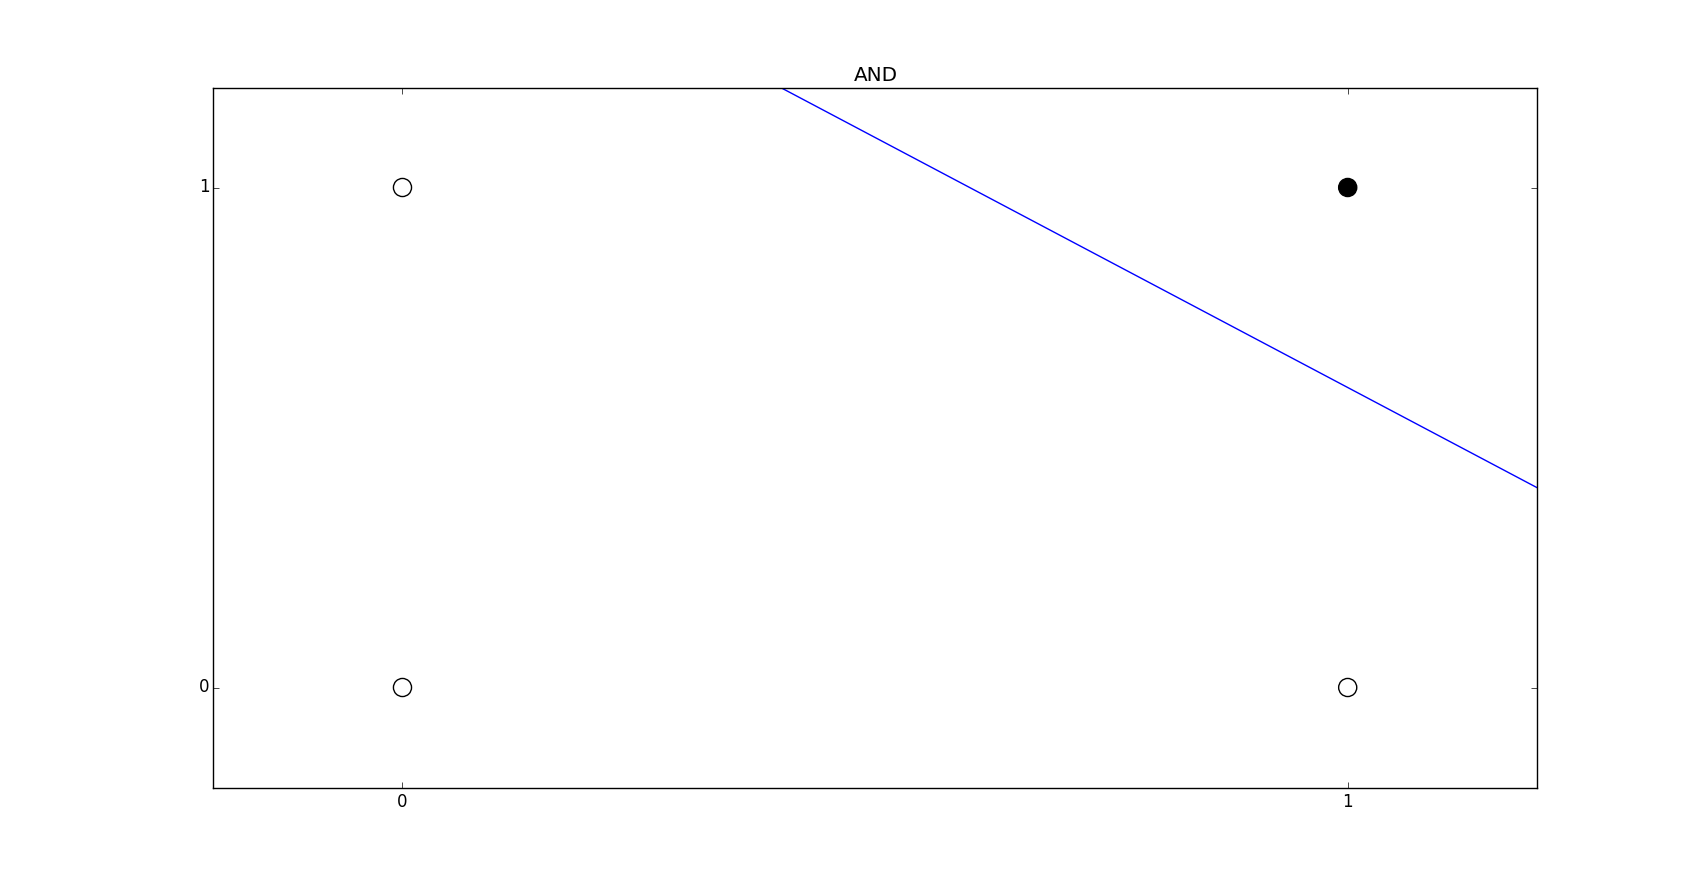
\includegraphics[scale=0.25]{pictures/and.png}
  \end{center}
\end{frame}

\begin{frame}
  \begin{center}
    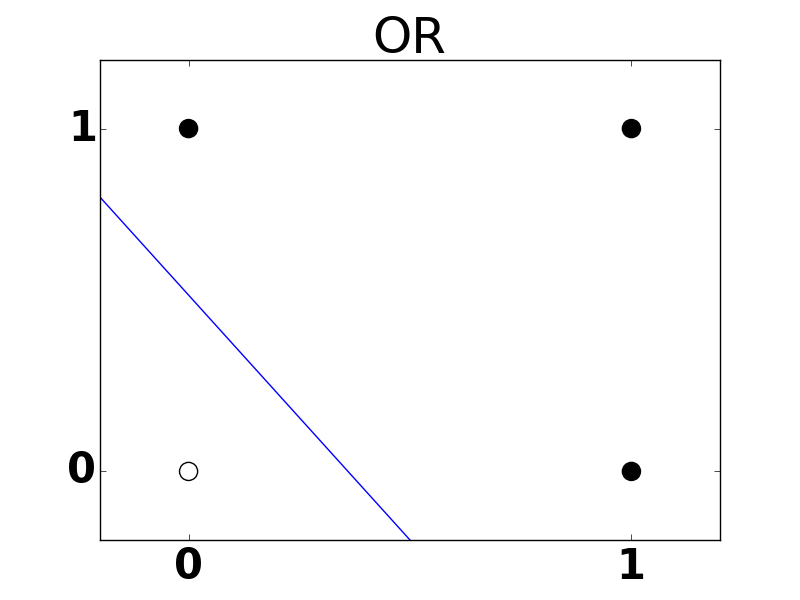
\includegraphics[scale=0.25]{pictures/or.png}
  \end{center}
\end{frame}

\begin{frame}
  \begin{center}
    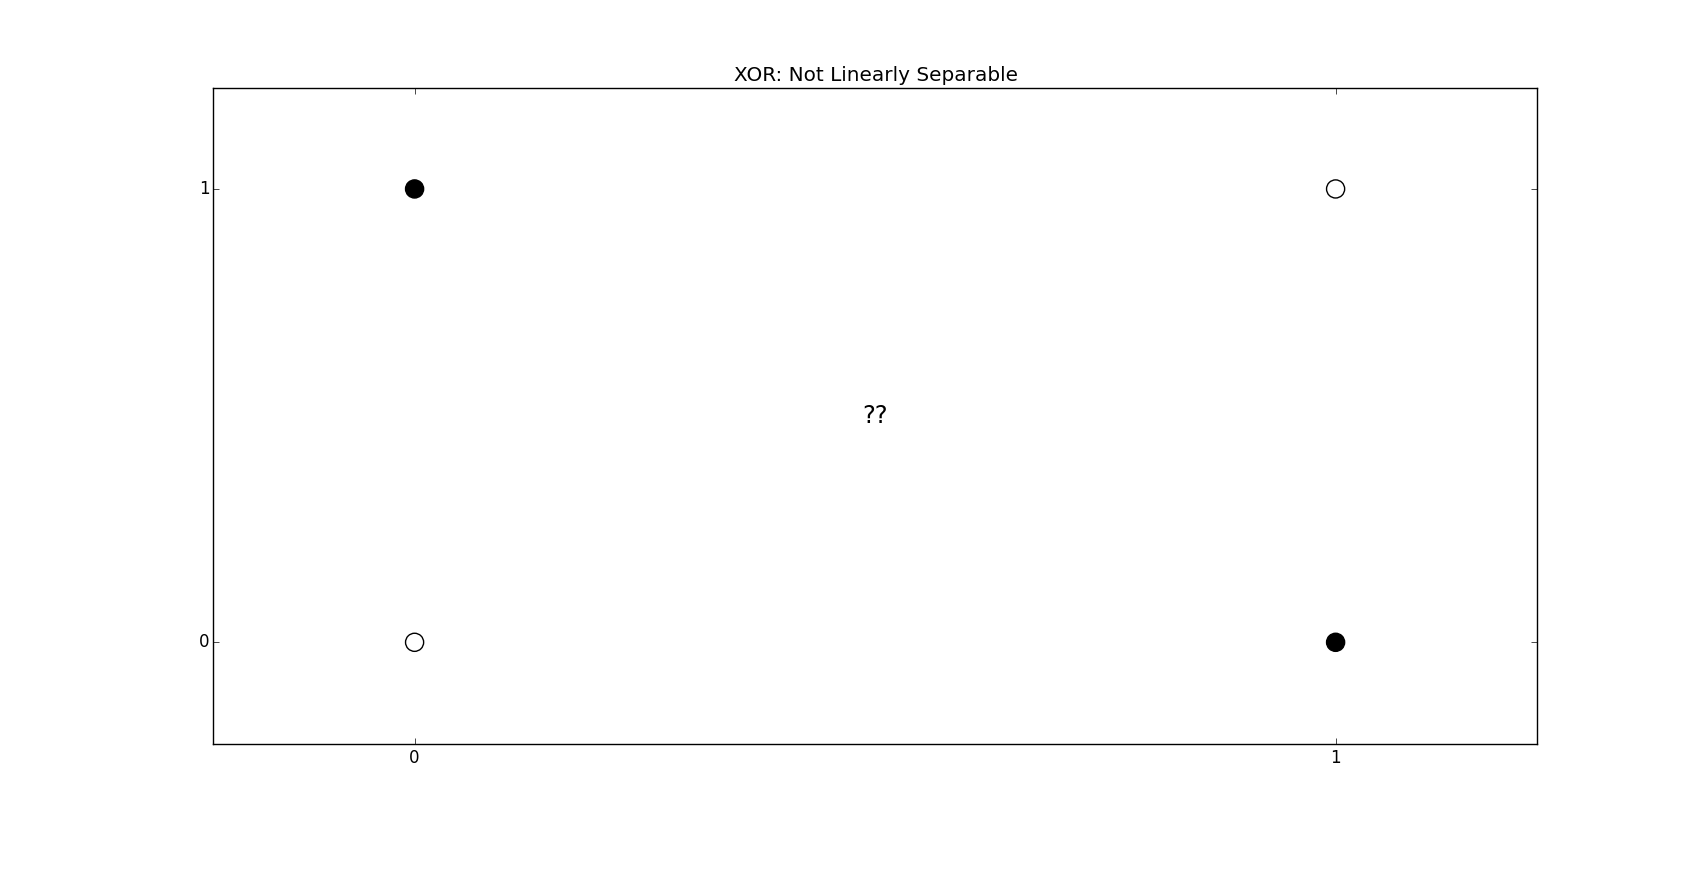
\includegraphics[scale=0.25]{pictures/xor.png}
  \end{center}
\end{frame}

\begin{frame}[fragile]
  \begin{block}{Forward propagation}
    \begin{lstlisting}
def add_bias(o):
    return insert(o, 0, 1, axis=0)
|\pause|
def h(x, w):
    out = [x]|\pause|
    for l in range(len(w)):|\pause|
        x = add_bias(out[l])|\pause|
        o = g(transpose(w[l]) * x)|\pause|
        out.append(o)|\pause|
    return out
  \end{lstlisting}
  \end{block}
\end{frame}
% Linearly separable data vs non-linearly separable data.


\begin{frame}
  \begin{center}
  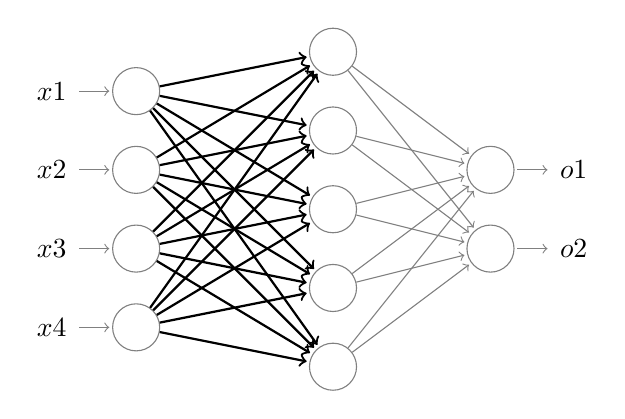
\begin{tikzpicture}[shorten >=1pt,->,draw=black!50, node distance=2.5cm]
    \tikzstyle{every pin edge}=[<-,shorten <=1pt]
    \tikzstyle{neuron}=[circle,draw,minimum size=17pt,inner sep=0pt]

    % input layer nodes
    \foreach \y in {1,...,4}
    \node[neuron, pin=left:$x\y$] (I-\y) at (0,-\y) {};

    % hidden layer nodes
    \foreach \y in {1,...,5}
    \path[yshift=0.5cm]
    node[neuron] (H-\y) at (2.5,-\y) {};

    % output layer node
    \foreach \y in {1,2}
    \path[yshift=-1cm]
    node[neuron,pin={[pin edge={->}]right:$o\y$}] (O-\y) at (4.5,-\y) {};

    % Connect every node in the input layer with every node in the
    % hidden layer.
    \foreach \src in {1,...,4}
    \foreach \dst in {1,...,5}
    \path[draw=black,thick] (I-\src) edge (H-\dst);

    % Connect every node in the hidden layer with the output layer
    \foreach \src in {1,...,5}
    \foreach \dst in {1,2}
    \path (H-\src) edge (O-\dst);
  \end{tikzpicture}
  \end{center}
\end{frame}

\begin{frame}
  \begin{center}
  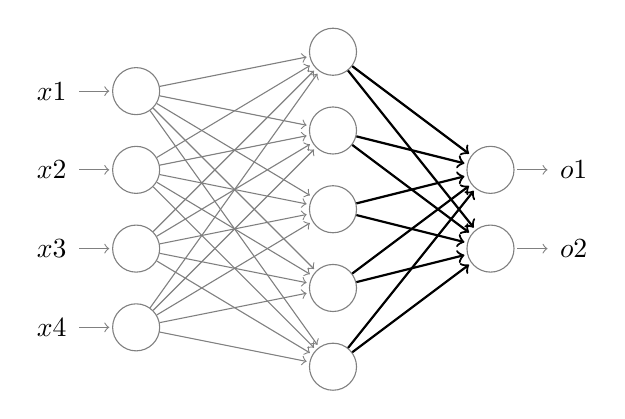
\begin{tikzpicture}[shorten >=1pt,->,draw=black!50, node distance=2.5cm]
    \tikzstyle{every pin edge}=[<-,shorten <=1pt]
    \tikzstyle{neuron}=[circle,draw,minimum size=17pt,inner sep=0pt]

    % input layer nodes
    \foreach \y in {1,...,4}
    \node[neuron, pin=left:$x\y$] (I-\y) at (0,-\y) {};

    % hidden layer nodes
    \foreach \y in {1,...,5}
    \path[yshift=0.5cm]
    node[neuron] (H-\y) at (2.5,-\y) {};

    % output layer node
    \foreach \y in {1,2}
    \path[yshift=-1cm]
    node[neuron,pin={[pin edge={->}]right:$o\y$}] (O-\y) at (4.5,-\y) {};

    % Connect every node in the input layer with every node in the
    % hidden layer.
    \foreach \src in {1,...,4}
    \foreach \dst in {1,...,5}
    \path (I-\src) edge (H-\dst);

    % Connect every node in the hidden layer with the output layer
    \foreach \src in {1,...,5}
    \foreach \dst in {1,2}
    \path[draw=black,thick] (H-\src) edge (O-\dst);
  \end{tikzpicture}
  \end{center}
\end{frame}

% if input is (x1, x2), add x1^2, x2^2 and x1x2 as inputs

\begin{frame}
  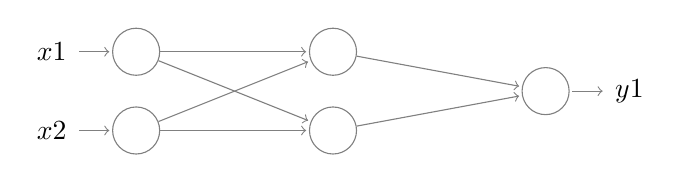
\begin{tikzpicture}[shorten >=1pt,->,draw=black!50, node distance=2.5cm]
    \tikzstyle{every pin edge}=[<-,shorten <=1pt]
    \tikzstyle{neuron}=[circle,draw,minimum size=17pt,inner sep=0pt]

    % input layer nodes
    \foreach \y in {1,...,2}
    \node[neuron, pin=left:$x\y$] (I-\y) at (0,-\y) {};

    % hidden layer nodes
    \foreach \y in {1,...,2}
    \path[yshift=0cm]
    node[neuron] (H-\y) at (2.5,-\y) {};

    % output layer node
    \foreach \y in {1}
    \path[yshift=-0.5cm]
    node[neuron,pin={[pin edge={->}]right:$y\y$}, right of=H-2] (O-\y) at (2.7,-\y) {};

    % Connect every node in the input layer with every node in the
    % hidden layer.
    \foreach \src in {1,...,2}
    \foreach \dst in {1,...,2}
    \path (I-\src) edge (H-\dst);

    % Connect every node in the hidden layer with the output layer
    \foreach \src in {1,...,2}
    \foreach \dst in {1}
    \path (H-\src) edge (O-\dst);
  \end{tikzpicture}
\end{frame}
